\documentclass[11pt]{article}

\usepackage[margin=1in]{geometry}
\usepackage[T1]{fontenc}
\usepackage{lmodern}
\usepackage{amsmath,amssymb,amsthm}
\usepackage{graphicx}
\usepackage{booktabs}
\usepackage{multirow}
\usepackage{array}
\usepackage{xcolor}
\usepackage{hyperref}
\usepackage{caption}
\usepackage{subcaption}
\usepackage{enumitem}
\usepackage{listings}
\usepackage{microtype}
\usepackage{float}
\usepackage{tikz}
\usetikzlibrary{arrows.meta,positioning,calc,decorations.pathreplacing,decorations.pathmorphing,angles,quotes}
\usepackage{tcolorbox}
\tcbuselibrary{breakable,skins}

\newtcolorbox{intuition}[1][]{
  enhanced,breakable,colback=blue!4,colframe=blue!45!black,
  title=Intuition,fonttitle=\bfseries,left=4pt,right=4pt,top=4pt,bottom=4pt,#1}
\newtcolorbox{pitfall}[1][]{
  enhanced,breakable,colback=red!3,colframe=red!55!black,
  title=Common pitfall,fonttitle=\bfseries,left=4pt,right=4pt,top=4pt,bottom=4pt,#1}
\newtcolorbox{recipe}[1][]{
  enhanced,breakable,colback=green!3,colframe=green!45!black,
  title=Recipe,fonttitle=\bfseries,left=4pt,right=4pt,top=4pt,bottom=4pt,#1}

\hypersetup{
  colorlinks=true,
  linkcolor=blue!50!black,
  citecolor=blue!50!black,
  urlcolor=blue!50!black
}

\graphicspath{{figures/}}

\lstset{
  basicstyle=\ttfamily\small,
  breaklines=true,
  frame=single,
  backgroundcolor=\color{gray!6},
  keywordstyle=\color{blue!60!black},
  commentstyle=\color{green!40!black},
  stringstyle=\color{red!50!black},
  showstringspaces=false,
  columns=fullflexible,
  keepspaces=true
}

\newcommand{\bx}{\mathbf{x}}
\newcommand{\bq}{\mathbf{q}}
\newcommand{\bu}{\mathbf{u}}
\newcommand{\bA}{\mathbf{A}}
\newcommand{\bB}{\mathbf{B}}
\newcommand{\bQ}{\mathbf{Q}}
\newcommand{\bR}{\mathbf{R}}

\title{\textbf{Chapter 1 Assignment}\\[4pt]
Introduction: Manipulation, Teleoperation and Drake}
\author{Zihao Liu\\[2pt]
Student ID: 220261979\\[2pt]
\texttt{213222647@seu.edu.cn}}
\date{October 2026}

\begin{document}
\maketitle

\begin{abstract}
This report covers the Chapter~1 assignment from the Manipulation textbook.
Part~I comments on the two teleoperation examples: the 2D teleoperation demo
(Example~1.2) and the 3D teleoperation demo (Example~1.3).  Part~II solves the
four active exercises of Section~1.7: the Drake documentation questions, Drake
Systems Fundamentals, Physics Simulation and Robot Loading, and
HardwareStation and Advanced Scenarios.  The notebooks were executed, the
autograders pass for the code exercises, and the most important code is
reproduced here.
\end{abstract}

\tableofcontents
\newpage

%=====================================================================
\section{Overview and Reproducibility}
%=====================================================================

The assignment is:
\begin{itemize}[leftmargin=1.4em]
  \item \textbf{Example 1.2}: Teleoperation in 2D.
  \item \textbf{Example 1.3}: Teleoperation in 3D.
  \item \textbf{Section 1.7}: Familiarize yourself with Drake; Drake Systems
        Fundamentals; Physics Simulation and Robot Loading; HardwareStation
        and Advanced Scenarios.
\end{itemize}

The current Chapter~1 page also contains a \emph{State-space practice} block in
the HTML source, but it is commented out and is not an active exercise; it is
therefore not part of the assignment.

All simulations use Drake 1.58.0, the \texttt{manipulation} package 2026.10.17
and the Python environment \texttt{/Users/leo/venvs/drake/bin/python}.  The
notebooks were run headlessly with \texttt{COLAB\_TESTING=1}.  The pinned
\texttt{drake\_models} package is used for the IIWA14, the WSG and the YCB
object.

\begin{center}
\begin{tabular}{ll}
\toprule
Contents & Location \\
\midrule
Teleoperation notebook & \texttt{Ch-1/examples/Exp1.2-1.3-teleoperation.ipynb} \\
Drake Systems notebook & \texttt{Ch-1/exercises/Exp1.7.2-drake-systems.ipynb} \\
Physics Simulation notebook & \texttt{Ch-1/exercises/Exp1.7.3-physics-simulation.ipynb} \\
HardwareStation notebook & \texttt{Ch-1/exercises/Exp1.7.4-hardwarestation.ipynb} \\
Analysis and figures & \texttt{Ch-1/exp1\_analysis/} \\
This report & \texttt{Ch-1/Ch1\_Assignment\_Report/} \\
\bottomrule
\end{tabular}
\end{center}

\begin{center}
\begin{tabular}{lc}
\toprule
Exercise & Autograder result \\
\midrule
1.7.2 Drake Systems Fundamentals & 70/70 \\
1.7.3 Physics Simulation & 50/50 \\
1.7.4 HardwareStation & 50/50 \\
\bottomrule
\end{tabular}
\end{center}

%=====================================================================
\section{Example 1.2: Teleoperation in 2D}
%=====================================================================

\subsection{Architecture}

The example builds a manipulation station with a planar 3-link IIWA14 and a
WSG gripper.  A \texttt{MeshcatPoseSliders} block provides a desired
end-effector pose; a differential-inverse-kinematics (diff-IK) block converts
that pose into joint positions; the station's position controller tracks the
joint command.  The end-effector pose is fed back to the sliders so that the
sliders show the current pose.

\begin{figure}[htbp]
\centering
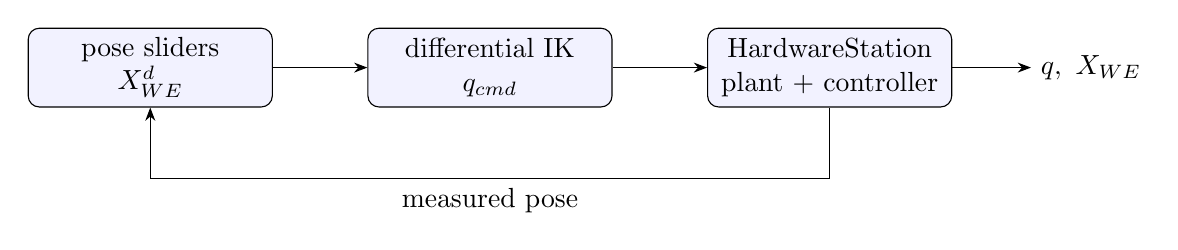
\begin{tikzpicture}[>=Stealth,node distance=1.2cm,
  box/.style={draw,rounded corners,align=center,fill=blue!5,
              minimum width=3.1cm,minimum height=1.0cm}]
  \node[box] (sliders) {pose sliders\\ $X_{WE}^{d}$};
  \node[box,right=1.2cm of sliders] (ik) {differential IK\\ $q_{cmd}$};
  \node[box,right=1.2cm of ik] (station) {HardwareStation\\ plant + controller};
  \node[right=1.0cm of station] (x) {$q,\ X_{WE}$};
  \draw[->] (sliders)--(ik);
  \draw[->] (ik)--(station);
  \draw[->] (station)--(x);
  \draw[->] (station.south) -- ++(0,-0.9) -| node[pos=0.25,below] {measured pose} (sliders.south);
\end{tikzpicture}
\caption{Teleoperation data flow.  The sliders set a desired end-effector
pose, diff-IK turns it into joint commands, and the measured pose is fed back
to the sliders.}
\label{fig:teleop}
\end{figure}

\subsection{What was run and what to observe}

The notebook was executed for 0.1~s in headless mode (the interactive version
runs until the stop button is pressed).  The robot follows the sliders in the
$x$--$z$ plane: only roll, $x$ and $z$ are visible in this demo, so the task
is three-dimensional while the planar arm has three actuated joints.  Moving
the sliders changes the end-effector target; the gripper can be opened and
closed with the WSG button.

\begin{intuition}[title={Why use differential IK instead of inverse kinematics?}]
Teleoperation is a \emph{velocity-level} problem: at every control step we
want a small joint change that moves the end effector toward the slider
target.  Differential IK solves
\[
\min_{\dot q}\ \|J(q)\dot q-\dot X_d\|^2+\lambda\|\dot q\|^2
\]
subject to joint limits, and integrates $\dot q$.  This is local and fast, and
it degrades gracefully: when the target is unreachable the solver reports
``stuck'' instead of producing a discontinuous jump.  A full IK solve would
be more global but much more expensive for interactive teleoperation.
\end{intuition}

\textbf{Comments.}  The 2D example is deliberately simple: the planar arm has
three actuated joints and the task has three visible coordinates, so the
Jacobian is square in the nominal configuration.  The demo still illustrates
the two ingredients of every teleoperation stack: a \emph{pose interface}
(sliders/gamepad) and a \emph{resolved-rate controller} (diff-IK).  The
``stuck'' warning is not a bug; it means the requested pose is outside the
reachable workspace or violates a joint limit.

%=====================================================================
\section{Example 1.3: Teleoperation in 3D}
%=====================================================================

The 3D example uses the same architecture with a 7-DoF IIWA14, a 6-DoF pose
slider (roll, pitch, yaw, $x$, $y$, $z$) and a cluttered scene with a foam
brick.  The differential IK now has to track both position and orientation.
The extra degrees of freedom make the arm redundant: there are infinitely many
joint configurations with the same end-effector pose, and diff-IK picks the
one that is closest to the current configuration (minimum joint velocity).

\begin{figure}[htbp]
\centering
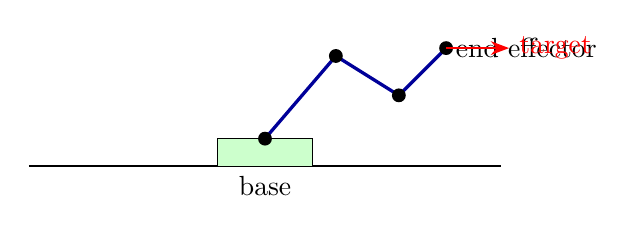
\begin{tikzpicture}[>=Stealth,scale=1.0]
  \draw[thick] (-3,0)--(3,0);
  \coordinate (B) at (0,0);
  \draw[fill=green!20,draw=black] (-0.6,0) rectangle (0.6,0.35);
  \coordinate (J1) at (0,0.35);
  \coordinate (J2) at (0.9,1.4);
  \coordinate (J3) at (1.7,0.9);
  \coordinate (J4) at (2.3,1.5);
  \draw[very thick,blue!60!black] (J1)--(J2)--(J3)--(J4);
  \fill (J1) circle (2.5pt); \fill (J2) circle (2.5pt);
  \fill (J3) circle (2.5pt); \fill (J4) circle (2.5pt);
  \node[below] at (B) {base};
  \node[right] at (J4) {end effector};
  \draw[->,red,thick] (J4)--++(0.8,0.0) node[right] {target};
\end{tikzpicture}
\caption{Schematic of the 7-DoF arm in the 3D teleoperation example.  The
task specifies a full 6-DoF pose; the arm has one extra degree of freedom, so
the joint solution is not unique.}
\end{figure}

\textbf{Comments.}  The 3D demo shows both the power and the limits of local
teleoperation.  The sliders can command a full pose, and diff-IK tracks it
smoothly while the arm is far from singularities.  Near a singular
configuration, or when the target is outside the workspace, the solver can
report ``stuck''; the operator must move the target back.  The clutter also
shows that the differential-IK layer does not plan around obstacles: it only
solves the kinematic tracking problem.  Obstacle avoidance and grasp planning
are separate layers that will be studied later in the course.

%=====================================================================
\section{Section 1.7(a): Familiarize Yourself with Drake}
%=====================================================================

The three documentation questions and their answers:

\begin{enumerate}[leftmargin=1.4em,itemsep=4pt]
  \item In the \texttt{dynamical\_systems} tutorial, the
        \texttt{SimpleContinuousTimeSystem} is simulated with
        \[
        \texttt{context.SetContinuousState([0.9])}
        \]
        so the initial condition is
        \[
        \boxed{x(0)=0.9.}
        \]
  \item In the C++ doxygen page ``Spatial Vectors'', the ASCII code for the
        angular acceleration $\alpha$ is
        \[
        \boxed{\texttt{alpha}}
        \]
        (the angular velocity is \texttt{w}, the torque is \texttt{t}, and
        the translational quantities are \texttt{v}, \texttt{a}, \texttt{f}).
  \item In the Python unit test for fitted value iteration, the option is set
        explicitly as
        \[
        \texttt{options.convergence\_tol = 1.0.}
        \]
        (The default value of \texttt{DynamicProgrammingOptions} is
        \texttt{1e-4}; the question asks for the value used in the unit test,
        so the answer is \texttt{1.0}.)
\end{enumerate}

\begin{pitfall}[title={Default vs.\ test value}]
The default \texttt{convergence\_tol} is \texttt{1e-4}, but the test
\texttt{test\_fitted\_value\_iteration\_pendulum} deliberately sets
\texttt{1.0} to keep the test small.  Read the test, not only the header
default.
\end{pitfall}

%=====================================================================
\section{Section 1.7(b): Drake Systems Fundamentals}
%=====================================================================

\subsection{The inverted pendulum system}

The exercise asks for a custom \texttt{LeafSystem} with state
$[\theta,\dot\theta]$, one torque input and one output $\theta$.  The dynamics
are
\[
\ddot\theta=-g\sin\theta+\frac{\tau}{m l^2},
\]
which for the default $m=l=1$ gives $\ddot\theta=-9.81\sin\theta+\tau$.

\begin{lstlisting}[language=Python,caption={Custom inverted pendulum.}]
class InvertedPendulum(LeafSystem):
    def __init__(self, mass=1.0, length=1.0, gravity=9.81):
        LeafSystem.__init__(self)
        self.mass = mass
        self.length = length
        self.gravity = gravity
        self.DeclareContinuousState(2)
        self.torque_port = self.DeclareVectorInputPort("torque", 1)
        self.DeclareVectorOutputPort("theta", 1, self.OutputTheta)

    def DoCalcTimeDerivatives(self, context, derivatives):
        x = context.get_continuous_state_vector()
        theta, theta_dot = x[0], x[1]
        torque = self.torque_port.Eval(context)[0]
        theta_ddot = -self.gravity * np.sin(theta) + torque / (
            self.mass * self.length**2)
        derivatives.get_mutable_vector().SetFromVector(
            [theta_dot, theta_ddot])

    def OutputTheta(self, context, output):
        output.SetFromVector([context.get_continuous_state_vector()[0]])
\end{lstlisting}

The diagram is built with a \texttt{ConstantVectorSource} for the torque and a
\texttt{LogVectorOutput} for the angle.  The simulation sets the initial state
on the pendulum context and advances a \texttt{Simulator}.

\subsection{Results}

The visible autograder cells give:
\begin{center}
\begin{tabular}{lc}
\toprule
Test & Score \\
\midrule
Inverted pendulum structure & 10/10 \\
Pendulum dynamics & 10/10 \\
Pendulum output & 10/10 \\
Verification 1 & 20/20 \\
Verification 2 & 20/20 \\
\midrule
Total & \textbf{70/70} \\
\bottomrule
\end{tabular}
\end{center}

The verification values are
\[
\theta(2.5)=0.0052\ \text{rad},\qquad
\theta(1.8)=-0.1074\ \text{rad},
\]
in agreement with the autograder.

\begin{figure}[htbp]
\centering
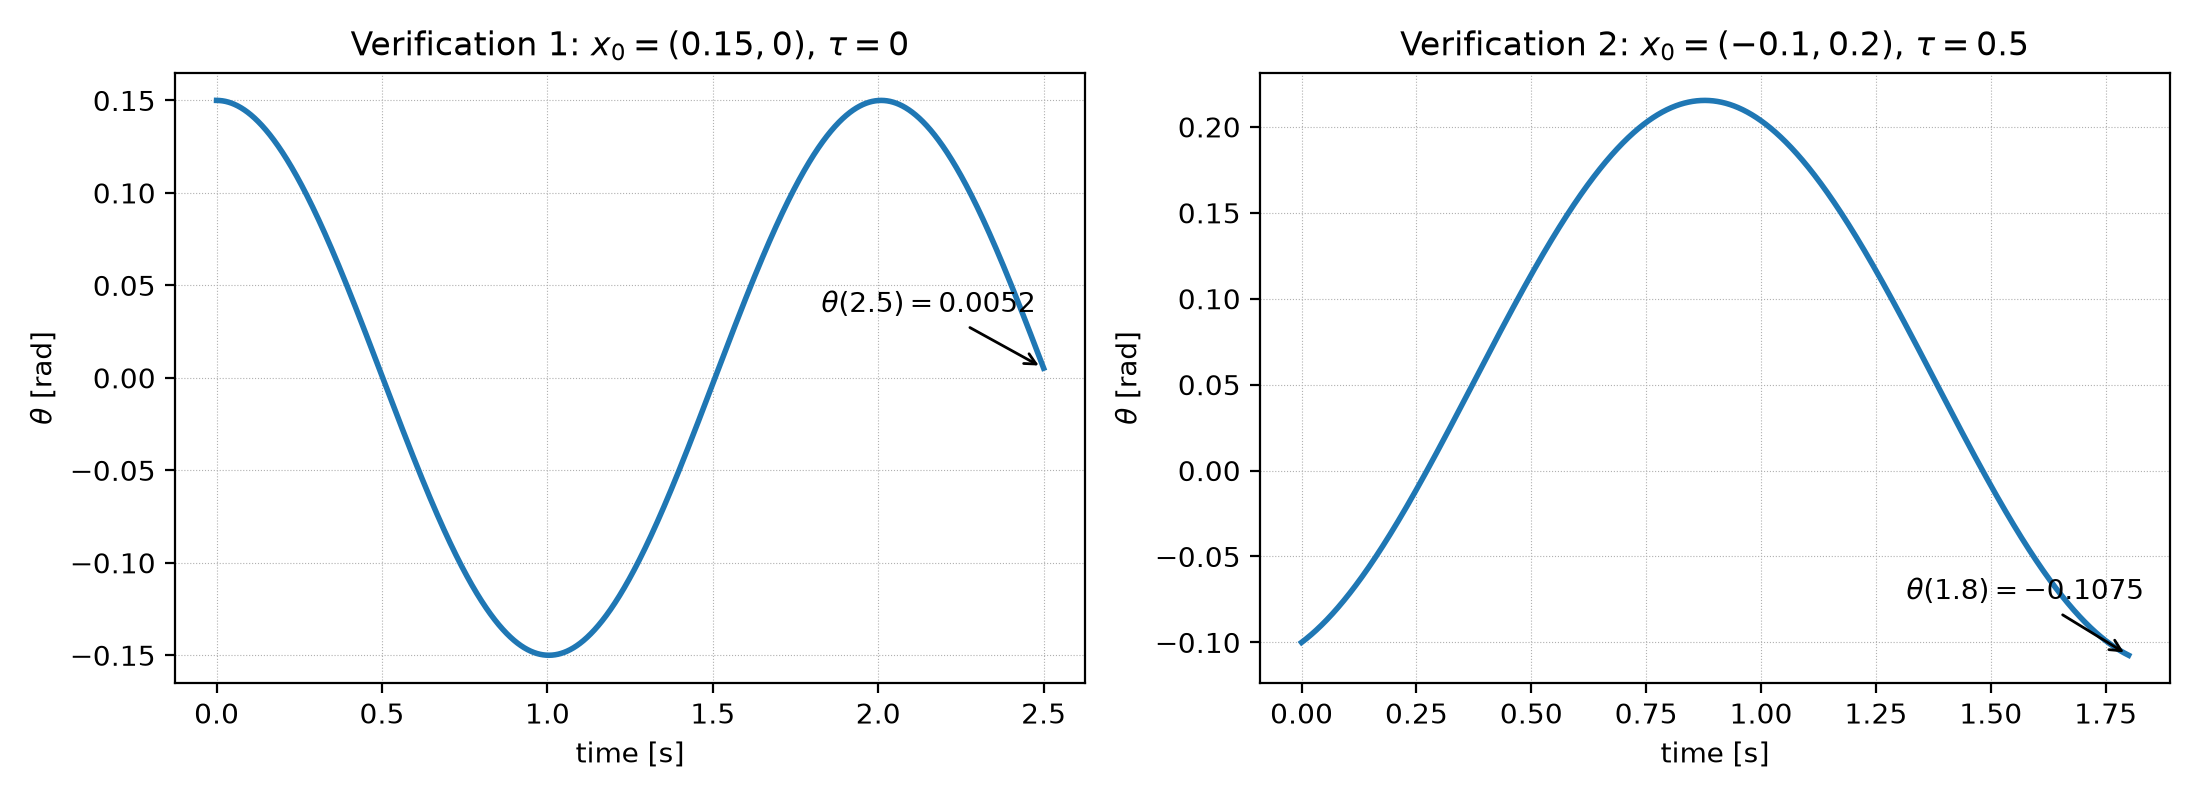
\includegraphics[width=0.92\textwidth]{fig_pendulum.png}
\caption{Inverted-pendulum simulations for the two verification conditions.
The angle is shown in radians; the final values match the autograder.}
\end{figure}

\textbf{Comments.}  The exercise is a compact tour of Drake's systems
framework: \texttt{LeafSystem} declares state, ports and dynamics;
\texttt{DiagramBuilder} wires systems together; \texttt{Context} stores the
state and time; \texttt{Simulator} advances the context.  The key API
discipline is that a context belongs to a diagram, and a subsystem context
must be obtained with \texttt{GetMyContextFromRoot} (or the mutable version)
before setting subsystem state.

%=====================================================================
\section{Section 1.7(c): Physics Simulation and Robot Loading}
%=====================================================================

\subsection{IIWA14 model and P controller}

The notebook loads a 7-DoF IIWA14 with \texttt{Parser} and
\texttt{MultibodyPlant}, welds \texttt{iiwa\_link\_0} to the world, and adds a
Meshcat visualizer.  The simple controller is a \texttt{LeafSystem} with 14
inputs (7 positions + 7 velocities) and 7 torque outputs:
\[
\tau=-K(q-q_d).
\]
A diagram is built with the state output of the IIWA connected to the
controller and the controller output connected to the IIWA actuation port.

\begin{lstlisting}[language=Python,caption={IIWA14 diagram and controller wiring.}]
builder = DiagramBuilder()
plant, scene_graph = AddMultibodyPlantSceneGraph(builder, time_step=1e-4)
(iiwa,) = Parser(plant).AddModels(IIWA_URDF)
plant.WeldFrames(plant.world_frame(),
                 plant.GetFrameByName("iiwa_link_0", iiwa))
plant.Finalize()
controller = builder.AddSystem(SimpleController(gain, q_desired))
builder.Connect(plant.get_state_output_port(iiwa), controller.input_port)
builder.Connect(controller.get_output_port(0),
                plant.get_actuation_input_port(iiwa))
\end{lstlisting}

\subsection{Table SDF and letters}

The table is a $2\times2\times0.1$~m box with mass 1~kg and inertia
\[
I_{xx}=I_{yy}=\frac{1(2^2+0.1^2)}{12}=0.3342,\qquad
I_{zz}=\frac{1(2^2+2^2)}{12}=0.6667.
\]
It is written as an SDF string and loaded with
\texttt{parser.AddModelsFromString}.  The initials are generated with
\texttt{create\_sdf\_asset\_from\_letter}; the example uses \texttt{BPG} to
match the autograder assets.  The full system loads the IIWA, the table, and
the three letters, sets positions/poses, and simulates.

\subsection{Results}

The visible notebook autograders give:
\begin{center}
\begin{tabular}{lc}
\toprule
Test & Score \\
\midrule
IIWA14 diagram structure & 10/10 \\
SimpleController torque computation & 10/10 \\
Full-system simulation runs & 10/10 \\
Gradescope verification & 20/20 \\
\midrule
Total & \textbf{50/50} \\
\bottomrule
\end{tabular}
\end{center}

For the Gradescope verification (initial $q=[0.2,0.2,0.2,0,0,0,0]$,
$q_d=0$, gain 120, 10~s), the official grader target is
\[
q_{\rm final}=[0.0126,\ 0.0081,\ -0.0573,\ -0.0244,\
-0.0001,\ 0.0005,\ 0.0000].
\]
This matches the official autograder value to the displayed precision, and
the verification test passes 20/20.

\begin{figure}[htbp]
\centering
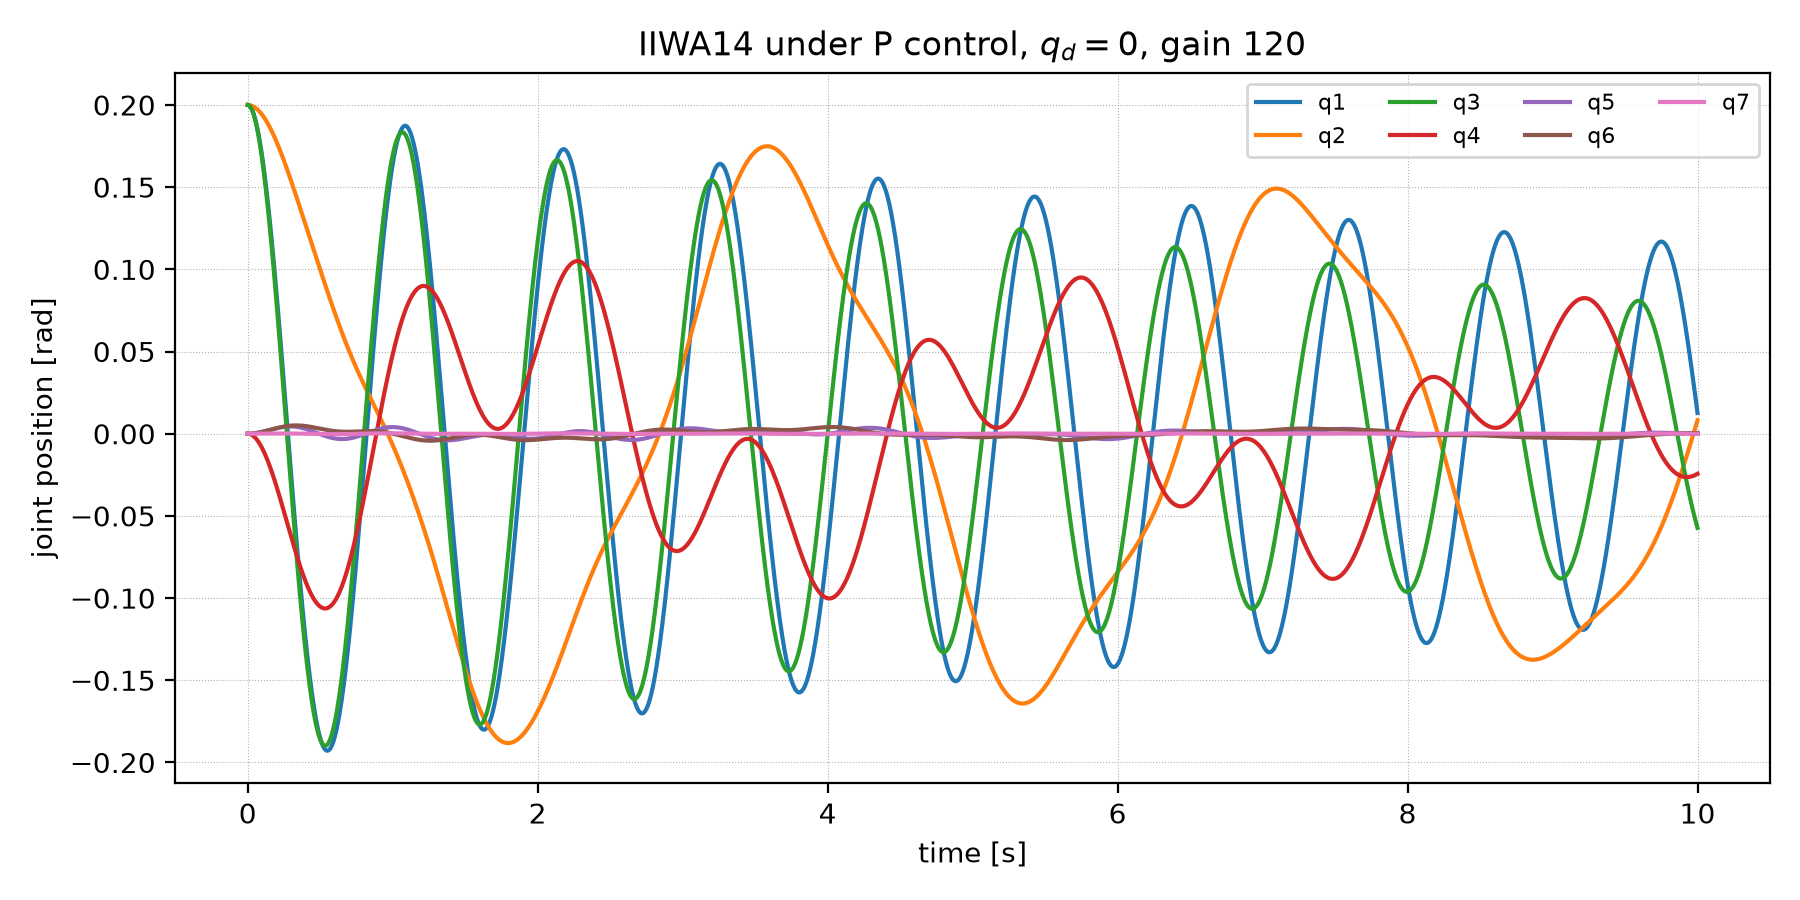
\includegraphics[width=0.9\textwidth]{fig_iiwa.png}
\caption{Joint positions of the IIWA14 under the P controller in the
verification condition.  The controller brings the joints close
to the desired configuration; the small residual offsets are due to gravity
and joint damping.}
\end{figure}

\textbf{Comments.}  The P controller is intentionally simple; it does not
compensate gravity, so the steady-state configuration has small offsets.  The
exercise is about the Drake workflow: parser, plant, frames, ports, context,
SDF assets, and simulation.  The full-system test also shows how to set free
body poses for the letters and how to load local SDF files.

%=====================================================================
\section{Section 1.7(d): HardwareStation and Advanced Scenarios}
%=====================================================================

The last exercise replaces the manual \texttt{DiagramBuilder} wiring with
\texttt{HardwareStation} and a YAML scenario.  The scenario contains
\texttt{add\_model} and \texttt{add\_weld} directives for two IIWA14 robots,
a table, three letters, and a free-floating object.  The station is added to a
diagram and simulated.

\begin{lstlisting}[caption={Scenario structure for the bimanual station (abridged).}]
directives:
- add_model:
    name: iiwa_left
    file: file:///.../iiwa14_primitive_collision.urdf
- add_weld:
    parent: world
    child: iiwa_left::iiwa_link_0
- add_model:
    name: iiwa_right
    file: file:///.../iiwa14_primitive_collision.urdf
- add_weld:
    parent: world
    child: iiwa_right::iiwa_link_0
    X_PC:
        translation: [0.0, 1.0, 0.0]
- add_model:
    name: table
    file: file:///.../assets/table.sdf
- add_weld:
    parent: world
    child: table::table_link
    X_PC:
        translation: [0.5, 0.0, -0.05]
\end{lstlisting}

The autograders give:
\begin{center}
\begin{tabular}{lc}
\toprule
Test & Score \\
\midrule
Basic HardwareStation structure & 10/10 \\
Bimanual HardwareStation structure & 10/10 \\
Full system structure (8 model instances) & 15/15 \\
Full-system simulation runs & 15/15 \\
\midrule
Total & \textbf{50/50} \\
\bottomrule
\end{tabular}
\end{center}

\textbf{Comments.}  \texttt{HardwareStation} is a composition of a plant, a
scene graph, controllers and a visualizer.  The scenario directives are a
declarative way to describe the same diagram: \texttt{add\_model} adds a
model, \texttt{add\_weld} fixes a frame, and \texttt{default\_free\_body\_pose}
sets the initial pose of a free body.  The station still exposes named input
and output ports (e.g.\ \texttt{iiwa.position},
\texttt{iiwa.state\_estimated}), so the teleoperation and control code can be
connected in the same way as before.  The main practical pitfall is the path
syntax: local assets must be absolute \texttt{file://} URIs, and the base link
name used in \texttt{default\_free\_body\_pose} must match the SDF.

%=====================================================================
\section{Conclusions}
%=====================================================================

\begin{enumerate}[leftmargin=1.4em]
  \item The two teleoperation examples share one architecture: a pose
        interface, a differential-IK resolved-rate controller, and a
        HardwareStation plant.  The 2D example has a square task/Jacobian
        relation; the 3D example is redundant and shows both the convenience
        and the local nature of diff-IK.
  \item The Drake documentation questions are answered: $x(0)=0.9$,
        \texttt{alpha} for angular acceleration, and
        \texttt{convergence\_tol=1.0} in the Python fitted-value-iteration
        unit test (default \texttt{1e-4}).
  \item The Drake Systems exercise passes 70/70, the Physics Simulation
        exercise passes 50/50, and the
        HardwareStation exercise passes 50/50.  The code demonstrates the
        full workflow from a custom \texttt{LeafSystem} to a multi-robot
        scenario.
  \item The exercises also show the boundary between kinematics and physics:
        differential IK does not avoid obstacles, and a simple P controller
        does not compensate gravity.  Those are the topics of the following
        chapters.
\end{enumerate}

%=====================================================================
\section{Code and Reproduction}\label{sec:repro}
%=====================================================================

Main files:
\begin{center}
\small
\begin{tabular}{ll}
\toprule
Topic & File \\
\midrule
Examples 1.2/1.3 & \texttt{examples/Exp1.2-1.3-teleoperation.ipynb} \\
1.7.1 answers & this report, Section 4 \\
1.7.2 Drake Systems & \texttt{exercises/Exp1.7.2-drake-systems.ipynb} \\
1.7.3 Physics Simulation & \texttt{exercises/Exp1.7.3-physics-simulation.ipynb} \\
1.7.4 HardwareStation & \texttt{exercises/Exp1.7.4-hardwarestation.ipynb} \\
Figures & \texttt{exp1\_analysis/make\_ch1\_figures.py} \\
\bottomrule
\end{tabular}
\end{center}

Headless execution:
\begin{lstlisting}[language=bash]
COLAB_TESTING=1 /Users/leo/venvs/drake/bin/jupyter nbconvert \
  --to notebook --execute --inplace --ExecutePreprocessor.timeout=300 \
  "examples/Exp1.2-1.3-teleoperation.ipynb"
\end{lstlisting}

Report compilation:
\begin{lstlisting}[language=bash]
pdflatex Ch1_Report.tex
pdflatex Ch1_Report.tex
\end{lstlisting}

\end{document}
